\subsection{Deep Learning}
Deep learning is a branch of machine learning. The main difference between the use of machine learning and deep learning, is that machine learning is not suitable for handling raw data form. Instead a machine learning system often needs a feature extractor, that will generate a feature vector from the data that can be used as an input for the machine learning system.
Deep learning is based on different techniques that makes it able to handle that data in its raw form, mainly because of its structure.\citep{LeCun2015, Schmidhuber2015} Because of this the system will automatically detect the necessary representations needed for classification and detection. Neural network is a structure of deep learning which consists of different layers, that can be divided into a input-layer and an output-layer, with one or more hidden layers in between \citep{Schmidhuber2015}. The key aspect of these layers is that the features are not defined by programmers, but they are found and learned from raw data using a general–purpose learning procedure.\citep{LeCun2015} An example of the structure can be seen in figure \ref{fig:NN_structure}.   


\begin{figure} [H]
\centering
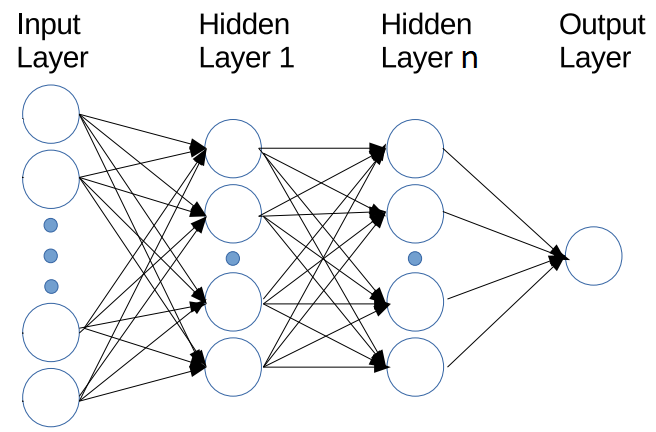
\includegraphics[width=0.6\textwidth]{figures/NN_structure}
\caption{Example of the neural network with possible layers\citep{Acquarelli2017}.}
\label{fig:NN_structure}  
\end{figure}

\noindent
The different layers consist of a series of nodes, where each node is connected by weights to one or several other nodes from a different layer. In the input-layer the nodes are fed with the data that the system is given. The second layer will then receive the output from the previous layer, and this process continues through the layers until the output-layer is reached.\citep{Schmidhuber2015} An example of how the hidden layers affect an image can be explained as follows:  
Firstly, the system detects minor changes like edges. Secondly, the edges are compared and put together to make up different kind of shapes. In the third hidden layer, it will be further combined to make up an object that can be identified.\citep{LeCun2015}

\subsubsection{Learning scenarios}
There are three main learning scenarios: supervised, unsupervised and semi-supervised learnings.

Supervised learning is the most common way of training in machine learning \citep{LeCun2015}. When using this method the system is trained with labeled data, where the generated output can be compared with an expected output, and thereby see evaluate the performance of the system. The weights are interconnection between two layers and they work as a set of coefficients, defining an image feature.\citep{Hameed2016} By adjusting weights in the neural network it is possible to fit the model better to the training data, and thereby increase its accuracy and reduce error \citep{LeCun2015}. Supervised learning is mostly associated with classification, regression, and ranking problems \citep{Mehryar2012}.
\noindent
Differently from supervised learning the input in unsupervised learning is received with unlabeled data and the predictions. Then the system organizes the data by searching for common characteristics \citep{Mehryar2012}. An example of an unsupervised learning algorithm is clustering, where the unlabeled dataset goes through a classification, and split into different classes.\citep{Goodfellow2016} 
\noindent
In semi-supervised learning the learner is receiving both labeled, unlabeled data and then it searches for common characteristics in data. It is used mainly when the labeled data is hardly collected and unlabeled data is easily reachable.\citep{Mehryar2012}


\subsubsection{Learning curves}
During the beginning of training, the training error of network will typically be relatively high, but during training the error decreases monotonically, as the weights are adjusted in the network \citep{Duda2000}. An illustration of how the error values are affected during training can be seen in \autoref{fig:learningCurve}.

\begin{figure} [H]
\centering
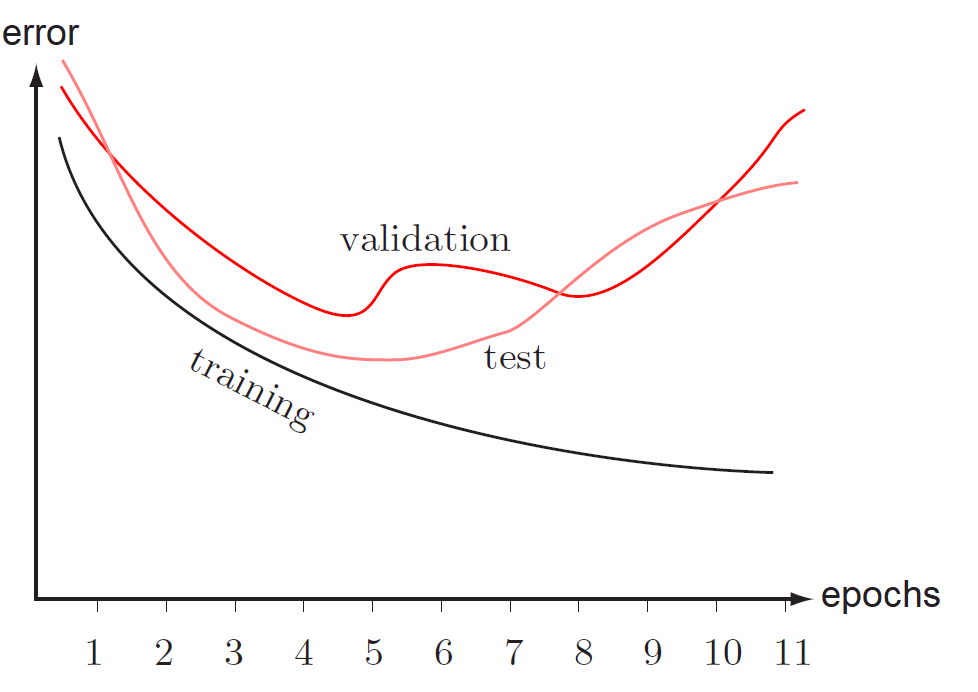
\includegraphics[width=0.7\textwidth]{figures/learningCurves}
\caption{Illustration of how training (black), validation (red), and test (orange) error is affected by the increase in epochs. Edited from \citep{Duda2000}.}
\label{fig:learningCurve}
\end{figure}

From the figure it can be seen how the error value of the validation, can be used to evaluate the network. 
Near the fifth epoch the validation and the test error starts to rise, indicating that the network is overfitting to the training data, thereby decreasing the generalization abilities. 
Validation error can therefor be used as stop criterion for when the training is optimal, and prevent overfitting. 
Typically the validation and test error will always be higher that the training error, which is also seen in \autoref{fig:learningCurve}. \citep{Duda2000}
  
\subsubsection{Back-propagation}
Backpropagation is a popular learning algorithm in neural networks, that is based on gradient decent, and valuable because of the simplicity and computationally efficient. \citep{Bengio2012, Duda2000}

Backpropagation is the process where the weights are adjusted to reduce the error between the input and desired output of the model. This also makes backpropagation the most general method used for supervised learning where the error is calculated through the used of the network's output and a real output.\citep{Duda2000} 

The different operating-phases of the can be split into a feedforward and learning phase. 
Feedforward is when the input is fed into the network and and output is given, simply by passing input through the different layers and weights. 
When the network is trained that weights are initiated with random values, from which the result is a low performance accuracy of the network. 
The learning phase is then again related to supervised learning, where parameters like the weights are adjusted to reduce error during training. \citep{Duda2000}
   

%er ved chap 6.3 i pattern 

In the backward process, weights will be updated to minimize the error between input and output layers.
This process will be applied until optimal weights with minimum error is reached.\citep{Hameed2016}


%Remember to write about batch and sochastic metods for traning with backprop

%Mention local minima and gobal minima and why it is not so importent to find the absolut global minima. 

%Explain gradient decent 

The basic idea behind it is to minimize the overall output error as much as possible during the learning stage. This algorithm process is divided in two main stages: forward and backward. In the first process (forward), the back-propagation architecture is described as  the inputs and weights multiplication of each node (separate input) summed with additional coefficients called biases.\citep{Hameed2016} 

\begin{comment}
It is defined by:
%H(j)=b_in+∑_(i=1)^N▒〖x_i w_ij 〗
Where: x – the inputs, i – neurons, w_ij – weights, j – neurons for hidden layer, b_in – biases
\end{comment}




%Additional info that need to be placed somewhere. 
\begin{itemize}
\item There are simple methods that can be used to improve performance and training speed. Scaling of the input and giving an initial weight \citep{Duda2000}

\item The architecture is important for classification, and depends on the given problem \citep{Duda2000}. 
\item  
\end{itemize}


\subsection{Convolutional Neural Networks}
Convolutional neural networks (CNNs) perform highly in several tasks, including digit recognition, image classification and face recognition. The key aspect of CNNs is to automatically learn a complex model by extracting visual features from the pixel-level content.
CNNs are feed–forward models that map input data with a set of suitable outputs. 
Accuracy and performance rely on large training datasets and training procedure based on back-propagation with optimization algorithm such as gradient descent which is used for finding minimum value of the function.\citep{Acquarelli2017}




